\documentclass[]{article}

%Language settings
\usepackage[spanish]{babel}

%Paper size and margins
\usepackage[letterpaper,top=2.54cm,bottom=2.54cm,left=2.54cm,right=2.54cm,marginparwidth=1.75cm]{geometry}

%Other packages
\usepackage{amsmath}
\usepackage{graphicx}
\usepackage[colorlinks=true, allcolors=blue]{hyperref}

\title{1. Divisor de voltaje}
\author{Flores Tun, Jorge David; López Gómez, Wilberth Eduardo; Sánchez Soberanis, Felipe}

\begin{document}
\maketitle

\section{Introducción}

Mediante el uso de los teoremas de máxima transferencia de potencia y divisor de voltaje, se presentará un circuito cuya función es mantener encendido un foco ubicado en un 
arreglo de divisor de voltaje, procurando que el voltaje de caída en ese nodo sea menor a 2 V cuando éste se encienda. Para esta práctica, se empleó el software de SparkFun para 
simular el circuito antes de realizarlo, al igual que se empleó un número "n" de resistencias de un mismo valor tanto para la simulación como para el circuito físico con el fin de 
obtener el valor resistivo requerido para el circuito.

\section{Marco teórico}

\subsection{Circuito Equivalente de Thevenin}

Un circuito eléctrico de dos terminales puede ser simplificado a uno más sencillo equivalente, el cual es conocido como circuito equivalente de Thevenin (Figura 1), 
el cual consta de una fuente de voltaje y una resistencia de Thevenin $R_{TH}$, la cual estará expuesta a un voltaje $V_{TH}$. 

\begin{figure}
    \centering
    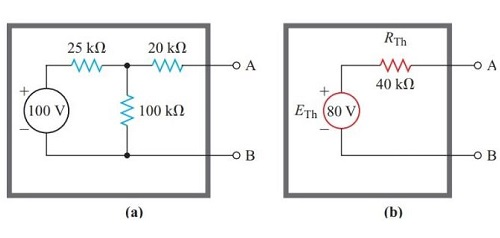
\includegraphics{build/Imagenes/CircuitoTH.jpg}
\end{figure}

\subsection{Teorema de la Máxima Transferencia de Potencia}

Cuando se tiene un circuito con dos terminales al que se le desea colocar una resistencia de carga $R_L$, con el fin de que se pueda 
transferir la máxima cantidad de potencia. El teorema de la máxima transferencia de potencia se da cuando se disipa la cantidad máxima de energía por medio de una resistencia de carga $R_L$ que es igual a la resistencia de Thevenin/Norton
del nodo donde se suministra el voltaje, por lo que da como respuesta una potencia disipada que será menor que la máxima. 

De igual manera, es importante recalcar que la potencia máxima no es equivalente a la máxima eficiencia en el sistema.

\subsection{Divisor de voltaje}

En un circuito, cuando se tiene un arreglo de resistencias, éstas se rigen por la ley de Ohm, la cual establece que:

\begin{equation*}
    V=IR 
\end{equation*}

Donde:
\begin{itemize}
    \item $I$ = Intensidad de corriente [A]
    \item R = Valor de la resistencia $[\Omega]$
    \item V = Voltaje [V]
\end{itemize}
    
Como todas las resistencias actúan de una misma manera, estan sometidas a la ley de Ohm, lo cual permite una serie de arreglos para poder hallar valores con mayor facilidad,
entre estos arrgelos, se encuentra el divisor de voltaje, la cual dicta que cuando se tiene un arreglo de dos resistencias $R_1$ y $R_2$ en serie de modo que se relacionan 
su voltaje de salida $v_{out}$ con el de entrada $v_{in}$, de modo que la ecuación queda de la siguiente manera:

\begin{equation*}
    V_{out}=(\frac{R_2}{(R_1+R_2)})*V_{in}
\end{equation*}

\section{Instrucciones}

Mediante un circuito constituido por una fuente, dos resistencias equivalentes y
la teoría de la division de voltaje y la máxima transferencia de energía, se
pretende diseñar un arreglo de $n$ resistencias para realizar el encendido de
un foco, el cual es generado mediante un encendido del cual no sufra una caida
de voltaje menor a 2 V.

\section{Materiales}

\begin{itemize}
    \item Fuente de voltaje que pueda brindar una alimentación de 20 V.
    \item Resistencias (varias).
    \item Foco
    \item Switch
    \end{itemize}


\section{Desarrollo}

Mediante la fórmula de divisor de voltaje, se obtuvo el número de resistencias necesarias 
para $R_1$ y $R_2$ y, para calcular el número de resistecias requeridas se desarrolló un código en MathLAB, el cual esta disponible en anexos.\\

Para la práctica, requeríamos de 14 resistencias de $100 \Omega$  y 14 de $150 \Omega$, de modo que la potencia requerida para éstas sea de 1W, 
Esto debido a que la potencia requerida para el foco es de 4.58W, de modo que el circuito queda como:
\clearpage

\begin{figure}
    \centering
    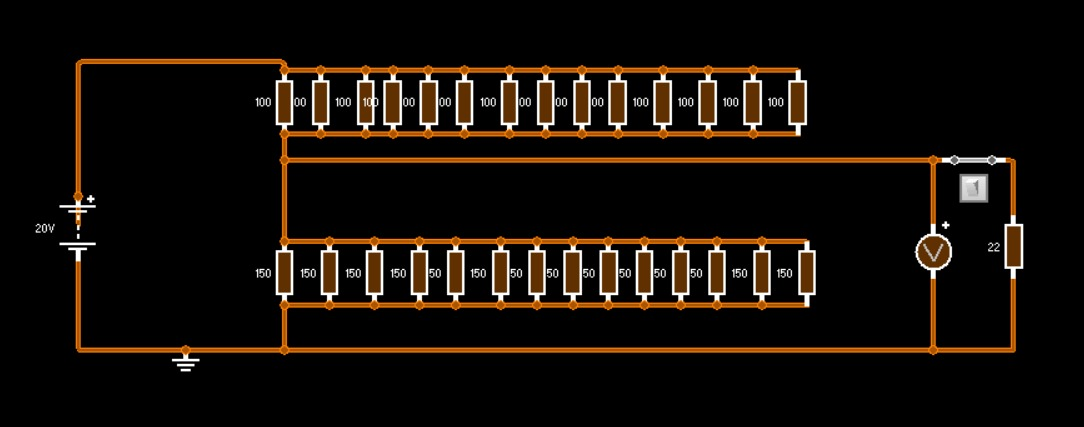
\includegraphics[width=8cm]{build/Imagenes/Circuito1.jpg}
    \caption{Figura 2: Diagrama del circuito en SparkFun}
\end{figure}
    
Sin embargo, para el ensamblado físico, en el protoboard no llegaba el voltaje apto para encender el foco, de igual manera que las resistencias variaban demasiado en el mismo, es 
por este motivo que se tuvo que implementar una resistencia más de 100 $\Omega$ para que pueda llegar a la resistencia deseada y se optó por unirlas de la siguiente manera:

\begin{figure}[htb]
    \centering
    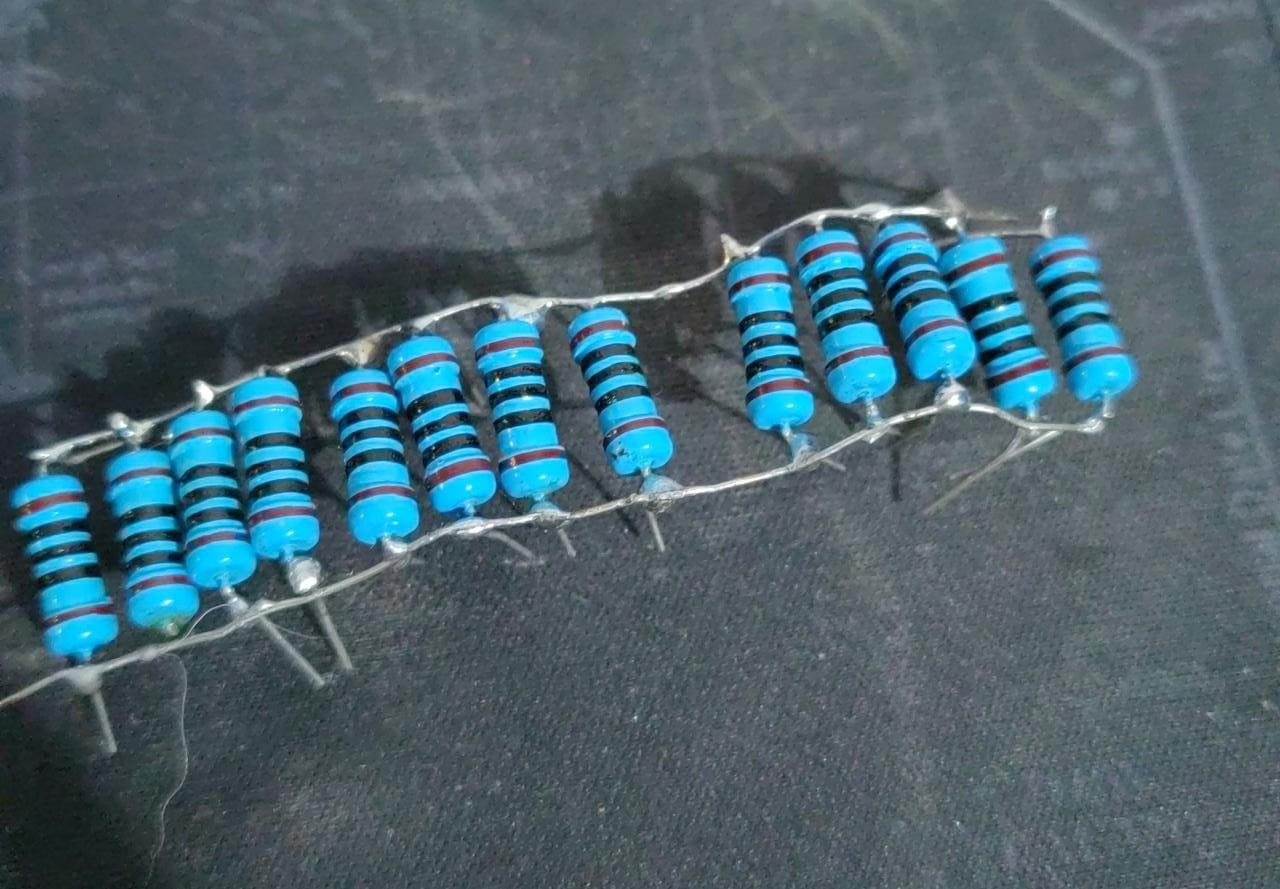
\includegraphics[width=8cm]{build/Imagenes/Resistencias.jpg}
    \caption{Figura 3:Configuración del sistema de resistencias}
\end{figure}

\section{Resultados}

Para la prueba, cuando el foco tenía circuito abierto, el voltaje que se obtuvo fue de 9.4 V, y cuando se realizó la conexión con el foco al circuito, se obtuvo una caida de voltaje
a 7.3 V, lo cual es un valor aproximado a 2V de caida, por lo que se cumplió con el objetivo de la práctica de no bajar más de 2V para la conexión del foco.

\section{Conclusiones}

La simulación es una gran alternativa para conocer el comportamiento de un circuito antes del armado físico, mas sin embargo, hay que tener en cuenta que la simulación es 
elaborada a base de un ambiente ideal, donde las resistencias no varían y la fuente brinda un valor de voltaje siempre constante en el tiempo, es por esto que en nuestro caso, 
la simulación maquilló de gran manera el comportamiento del circuito en físico, ya que tuvimos que recurrir a varios intentos antes de lograr el objetivo de la práctica, donde
tuvimos resistencias quemadas, con valores inexactos, al igual que en la simulación no se contemplaba como tal la potencia requerida de las resistencias, lo cual nos sumo más 
intentos, pero con esta práctica aprendimos como actúa el teorema de máxima transferencia de potencia en el ámbito práctico y la inexactitud de la simulación a la hora de representarla
en un medio físico.

\section{Anexos}
Código de MathLAB:

clear; clc;

syms R2 RL i i0;

R1 = 82/4;

RL = 22;

R2 = RL*R1./(R1-RL)

eqn1 = -20 + R1*i0 + R2*(i0 - i) == 0;
eqn2 = -R2*(i0 - i) + RL*i == 0;

[A, B] = equationsToMatrix([eqn1, eqn2], [i0, i]);

X = linsolve(A, B);

i0 = double(X(1))
i = double(X(2))

vfinal = i*RL
Wfinal = i*vfinal

VR2 = R2*(i0-i);
WR2 = VR2*(i0-i)

VR1 = R1*i0;
WR1 = VR1*i0

V1 = 9.75;
I1 = 500e-3;
R1 = V1 / I1

V2 = 7.64;
I2 = 1.6;
R2 = V2 / R2

V3 = 10.18;
I3 = 450e-3;
R3 = V3 / I3

\bibliographystyle{alpha}

\end{document}